

\documentclass{article}

\usepackage{amsmath}
\usepackage{graphicx}


\author{Qing Scholten, Wessel van Sommeren}
\title{Controlling a rabbit plaque}

\begin{document}

\maketitle
\newpage
\tableofcontents
\newpage

\section{Introduction}
In 1859 the First Fleet of settlers arrived in Australia, with them Thomas Austin. Thomas Austin took 13 European rabbits with him on his journey, so that once in Australia he could set them free so that he could hunt them for food. What Thomas Austin did not know was that these European rabbits did not have any natural predators or competition in australia. So by 1920 the small population of 13 rabbits had turned into a rabbit plaque, in 1920 there were an estimated 10 billion rabbits in australia.In this paper we will attempt to model the rabbit plaque of australia by exploring the question "What is the most effective way to control a rabbit plaque comparing Hunting, Introducing a predator and Introducing a Competitor 
\section{Base case}
For the base case we use the fact that a rabbit on average gets 4 - 8 babies per 60 days. So we take 6 on average that means one rabbit produces 0.1 rabbit per day. A rabbit in the wild live up to 9 nine years this means 0.000312109862672 rabbits die per day per rabbit. This means we get 
$$
\frac{dP(t)}{dt} = 0.1P(t)-0.000312109862672P(t)
$$

We take $P(0) = 13$ as starting population
\\

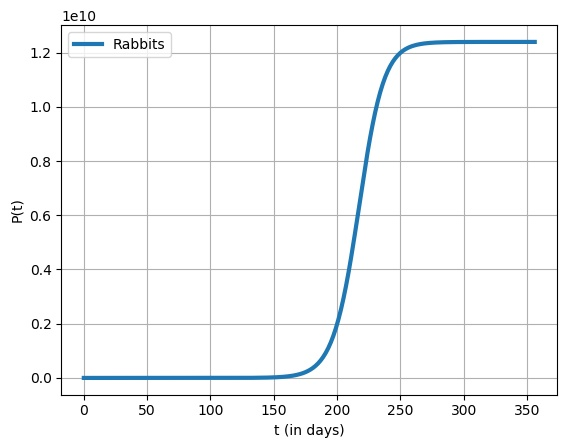
\includegraphics[scale=0.78]{Pictures/unr_rabbitts}
\\ 
As we can see from the graph de population of 13 rabbits grew to more than  $2.5\cdot10^{11}$ in just 250 days. This would continue to grow exponentially forever as the current model does not have a limiting factor. The limiting factor in our model is going to be food. As Australia has about 7 616 666 square kilometer land and 1 371 000 square kilometer of this land is desert, one finds that about 7 479 566 square kilometer is fertile land. This follows from the assumption that every land outside the deserts is able to grow grass, which is the vegetation that is used in the model. Known is that "the average annual total herbage production at Moorepark for the period 2005–9 was 14 087 kg DM/ ha, with an average grass growth of 50·3 kg DM/ha/day." A 1 hectare is equal to 0.01 square kilometer, the avarage annual total herbage production 140.87 kg $Dm/km^2$, so for Australia this is about 1 052 646 462 kg Dm. This means that the amount of grass, as grass has about 17 dry material, is about 6 197 920 367 kg grass for the whole of Australia. As rabbits eat around 1 cup of grass for 2 lbs of body weight, this would convert to about 0.25 kilo gram grass for a medium sized rabbit of 2 kilo gram. This means that Australia has enough grass to house 12 395 840 734 rabbits without running out of food.

Let $R$ be the reproduction number
$$
R = 0.1 - 0.000312109862672
$$
$$
\frac{dP(t)}{dt} = RP(t)(1-\frac{P}{12 395 840 734})
$$
\\
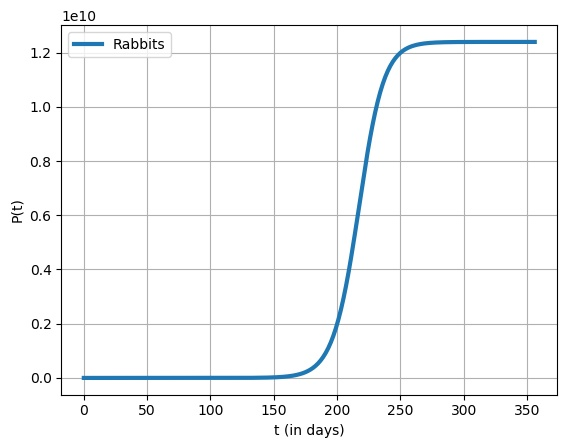
\includegraphics[scale=0.78]{Pictures/logis}
\\

From the graph we see that the model reaches an equilibrium around 12 395 840 734, which is what we expected and wanted. This can also be confirmed analytically 
$$
0= RP(t)(1-\frac{P(t)}{12 395 840 734})
$$
$$
RP(t) = 0
$$
$$
1-\frac{P(t)}{12 395 840 734} = 0
$$
$$
P(t) = 12 395 840 734
$$
This shows that the equilibrium solutions are 0 and 12 395 840 734
$$
M = 12 395 840 734 
$$
$$
\frac{dP(t)}{dt} = RP(t)(1 - \frac{1}{M}P(t))
$$
$$
\frac{dP(t)}{P(t)(1 - \frac{1}{M}P(t))} = Rdt
$$
$$
\frac{MdP(t)}{P(t)(M - P(t))} = Rdt
$$
$$
dP(t)(\frac{-1}{P(t)} - \frac{1}{M -P(t)})   = Rdt
$$
$$
\int{(\frac{1}{P(t)} - \frac{-1}{M -P(t)})dP(t) }  =\int{ R}dt
$$
$$
\ln(P(t)) - \ln(M -P(t)) + c_1 = Rt +c_2
$$

$$
 \ln(\frac{P(t)}{M -P(t)})  = Rt +c
$$

$$
\frac{P(t)}{M -P(t)}= e^{Rt +c}
$$

$$
P(t) = - \frac{Me^{Rt +c}}{1 - e^{Rt +c}}
$$
$$
P(0)(1 - e^{c}) = -Me^{c}
$$
$$
c = \ln(\frac{P(0)}{P(0)-M})
$$
$$
P(t) =  \frac{MP(0)}{P(0)+(M - P(0))e^{-Rt}}
$$
\section{Introducing a preditor: The Red Fox}
Australia 7 616 666 square kilometer land, of which 1 371 000 square kilometer is desert. Knowing that red foxes don't live in the desert, they have about 7 479 566 square kilometer land to live on. The red fox has a territory that ranges one to two miles from its home. Assuming that the territory of a red fox is circular with a radius of one mile, this means that the area a red fox needs is $\pi*1^2$ which is equal to about 3.14 square mile per fox. Converting this to square kilometer, the fox needs about 8.13 square kilometer of space. This means that Australia can house about 919 996 red foxes, without getting overcrowded. As foxes reproduce every 51 days and get on avarage 5 pups per two foxes, meaning that every fox wil get 2.5 pups in 51 days on avarage. This means that the birth rate is about 0.0245 pups per fox per day. Red foxes live nine years on avarage. This means that the death rate is about 0.0003044 deaths per fox per day.

Let $R_f$ be the reproduction number.
$$R_f = b_f - d_f$$
$$b_f = 0.0245$$
$$d_f = 0.0003044$$
$$\frac{dP_f(t)}{dt} = R_fP_f(t)(1-\frac{P_f(t)}{M_f})$$
$$M_f = 919996$$
\\
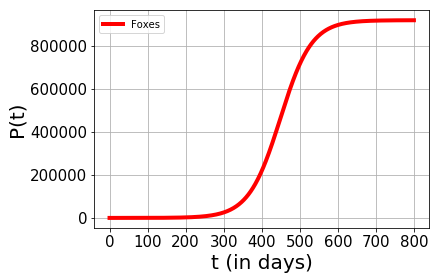
\includegraphics[scale=0.78]{Pictures/Foxes.png}
\\
From the graph we see that the model reaches an equilibrium around 919996, which is expected and wanted. This can also be confirmed analytically.
$$0=R_fP_f(t)(1-\frac{P_f(t)}{M_f})$$
$$R_fP_f(t)=0$$
$$1-\frac{P_f(t)}{M_f}=0$$
$$P_f(t)=M_f$$
$$P_f(t)=919996$$
This shows that the equilibrium solutions are 0 and 919996. In an equilibrium situation, the extra deathrate due to lack of space can be found by the following formula, as the extra deathrate is dependent on both the maximum amount of foxes and the growth rate of the amount of foxes.
$$\alpha_f = a_f * \overline{F}$$
Where $\alpha_f$ is $b_f-d_f$, $a_f$ is the extra deathrate on top of the constant deathrate due to space limitations and $\overline{F}$ is the amount of foxes in the equilibrium situation where
$$\overline{F} = 919996$$
This means that we can find the $a_f$ with the following formula
$$a_f = \frac{\alpha_f}{\overline{F}}$$
With this can be found that $a_f = 0.000000063$. The extra birthrate dependent on the amount of food (namely rabbits) available can be found by
$$\alpha_f + c_f*\overline{K}-a_f*\overline{F}=0$$
As the extra birthrate should be depend on the amount of rabbits, amount of foxes, the extra deathrate and the growth rate of the foxes, where $c_f$ is the extra birthrate dependent on the amount of food and $\overline{K}$ is the amount of rabbits in the equilibrium situation where
$$\overline{K}=12395840734$$
This means that we can find $c_f$ with the following formula
$$c_f=\frac{-\alpha+a_f*\overline{F}}{\overline{K}}$$
$$c_f=\frac{-\alpha+\frac{\alpha}{\overline{F}}*\overline{F}}{\overline{K}}$$
So we find that $c_f=0$. This means that the differential equation becomes 
$$\frac{dP_f(t)}{dt}=(b_f-d_f)*P_f*(1-\frac{P_f}{M_f}$$
We find that, as red foxes eat around 500 grams of food per day, a red fox eats about 0.25 rabbits a day when available, but their diet is dependent on how easy accessible the rabbits are, so more rabbits, means it's easier for the foxes to eat he rabbits. We find the extra deathrate due to foxes with the following formula, as this is dependent on the amount of foxes and the amount of rabbits.
$$a_k*\overline{F}*\overline{K}=0.25*\overline{F}$$
So we find now that we can find the extra deaths of rabbits due to foxes with
$$a_k=\frac{0.25}{\overline{K}}$$
Which means that $a_k=2.0168*10^{-11}$.
\\In the following graph the situation is plotted where there are 10000000000 rabbits and 919996 foxes, which is about the amount of rabbits Australia has when they had their big rabbit plague and the maximum amount of foxes that can live in Australia. In the graph one can see that due to the low maximum amount of foxes that can live in Australia, they don't do much to the rabbits, where they grow their amount to the equilibrium of $1.23935344*10^10$. The foxes have their equilibrium around $919996$. As the foxes only eat around 0.25 rabbit per fox at the most, they don't do much as a relatively small number of foxes can be housed in Australia in comparison to the amount of rabbits. 
\begin{center}
    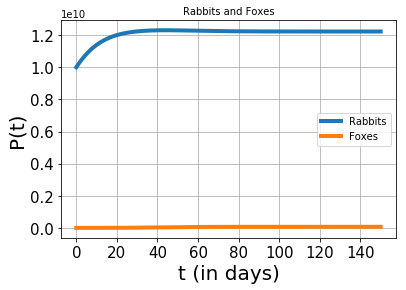
\includegraphics[scale=0.78]{Pictures/RabbitFoxes.png}
\end{center}


%https://cosleyzoo.org/red-fox/#:~:text=Shelter%20and%20Space%20Needs&text=The%20normal%20territory%20of%20the,remarkably%20to%20cohabitation%20with%20humans.
%https://ofnc.ca/programs/fletcher-wildlife-garden/flora-and-fauna-at-the-fwg/red-foxes-at-the-fwg
%https://www.nhm.ac.uk/discover/the-secret-life-of-urban-foxes.html#:~:text=Wild%20red%20foxes%20generally%20live,between%20one%20and%20three%20years.
%https://www.wildlifeonline.me.uk/animals/article/red-fox-diet-how-much-food#:~:text=Again%2C%20this%20is%20a%20deceptively,pound)%20of%20food%20per%20day.
%https://ofnc.ca/programs/fletcher-wildlife-garden/flora-and-fauna-at-the-fwg/red-foxes-at-the-fwg

\end{document}
